
\chapter{Resultados}
\label{cap:resultados}

Esta execução do pipeline cobre o ano de 2024. Das ocorrências desse ano,
\textbf{597 municípios} atingiram o volume mínimo de 30 ocorrências e entraram
na clusterização.

\section{Clusterização dos municípios}
\label{sec:resultado-cluster}

A \autoref{fig:silhouette} mostra o \textit{silhouette score} testado para $k$
de 2 a 8: o maior valor (aproximadamente 0,160) ocorre em $k=2$, caindo para
todos os demais valores testados, inclusive o segundo melhor, $k=4$
(aproximadamente 0,143). O pipeline escolheu, portanto, $\mathbf{k=2}$.

\begin{figure}[H]
  \centering
  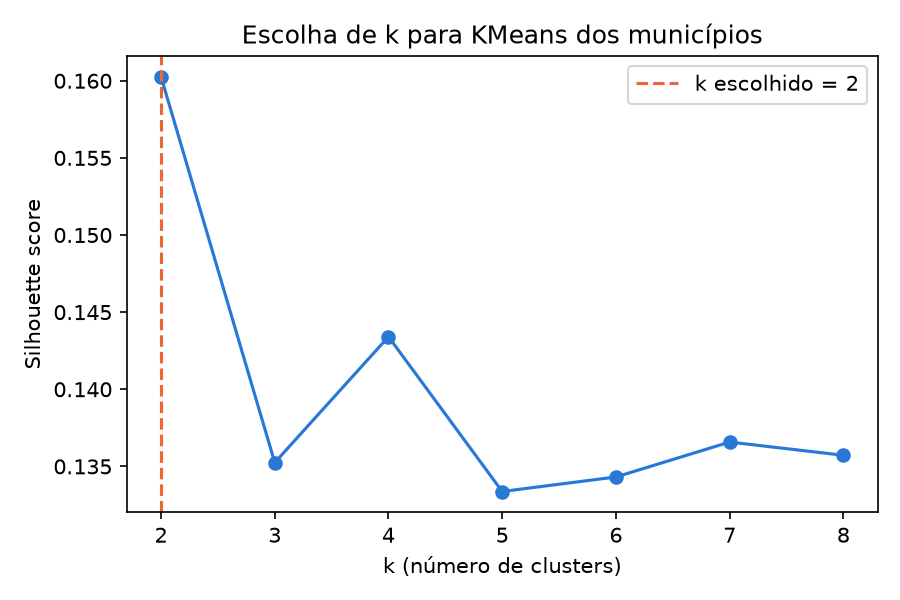
\includegraphics[width=0.34\textwidth]{./fig/ml_silhouette_k}
  \caption{Silhouette score por $k$ testado (2 a 8), ano de 2024.}
  \label{fig:silhouette}
  \fontefig{Elaborado pelo autor, a partir da saída do pipeline (\texttt{ml/output/silhouette\_por\_k.png})}
\end{figure}

O cluster 0 reúne 297 municípios e o cluster 1, 300: divisão praticamente
equilibrada em número de municípios, mas não em perfil de risco nem em
volume de ocorrências (\autoref{tab:perfil-cluster}).

\begin{table}[ht!]
\caption{Perfil médio por cluster de município, ano de 2024 (cluster 0: 297 municípios; cluster 1: 300 municípios)}
\label{tab:perfil-cluster}
\small
\begin{center}
\begin{tabular}{|l|c|c|}
\hline
\textbf{Métrica} & \textbf{Cluster 0} & \textbf{Cluster 1} \\
\hline
Ocorrências médias/município & 52,69 & 148,50 \\
\hline
Taxa de letalidade & 4,25\% & 2,12\% \\
\hline
Taxa de feridos graves & 12,19\% & 8,97\% \\
\hline
Veículos médios/ocorrência & 2,10 & 1,91 \\
\hline
Proporção fim de semana & 34,51\% & 31,69\% \\
\hline
Proporção período noturno & 5,12\% & 5,26\% \\
\hline
Proporção com chuva & 10,10\% & 12,07\% \\
\hline
Proporção pista simples & 88,40\% & 22,87\% \\
\hline
Concentração da causa principal & 20,90\% & 21,90\% \\
\hline
\end{tabular}
\end{center}
\fontetab{Elaborado pelo autor, a partir de \texttt{ml/output/clusters\_municipios.csv}}
\end{table}

\begin{itemize}
  \item \textbf{Cluster 0} ("Maior Letalidade"): \textbf{menor} volume
  médio (52,69 ocorrências/ano), via quase sempre de \textbf{pista simples}
  (88,40\%), \textbf{maior} taxa de letalidade (4,25\%, o dobro do cluster
  1) e de feridos graves (12,19\%). Perfil associado a vias simples/interestaduais;
  \item \textbf{Cluster 1} ("Menor Letalidade"): \textbf{maior} volume médio
  (148,50/ano, quase 3$\times$ o cluster 0), via predominantemente de
  \textbf{pista múltipla} (22,87\% de pista simples) e letalidade bem menor
  (2,12\%). Perfil de municípios maiores, com malha viária de maior
  capacidade.
\end{itemize}

\section{Regras de associação por cluster}
\label{sec:resultado-regras}

O cluster 0 reuniu 15.648 ocorrências e o cluster 1, 44.550, bases de
transações sobre as quais o Apriori rodou, separadamente. A
\autoref{fig:metabase-regras}, card do painel do Metabase, lista as cinco
regras de maior \textit{lift} de cada cluster ("Maior Letalidade" é o
cluster 0, "Menor Letalidade" o cluster 1; suporte e confiança em \%). A
lista completa, com até 15 regras por cluster, está em
\texttt{ml/output/regras\_associacao\_por\_cluster.csv}.

\begin{figure}[H]
  \centering
  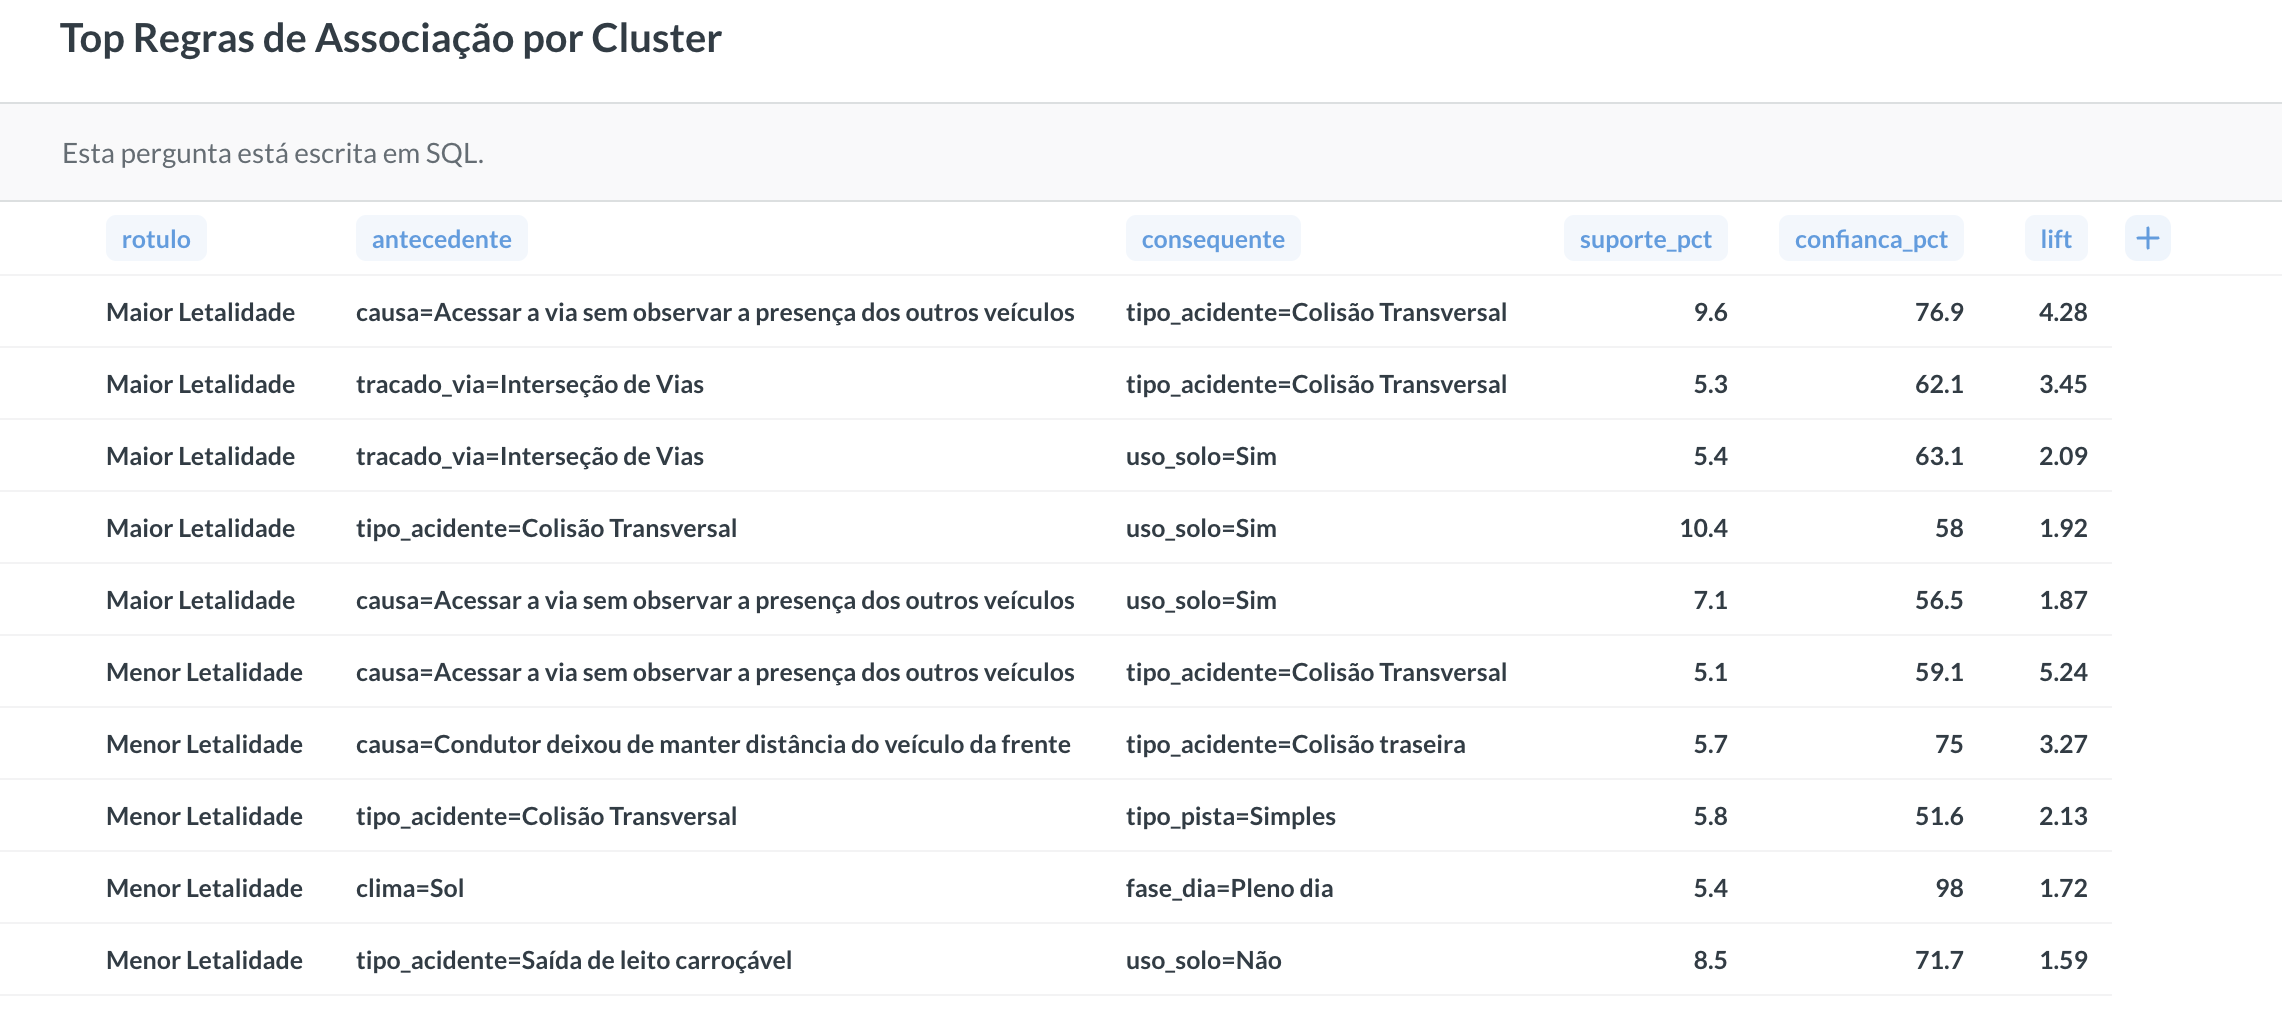
\includegraphics[width=\textwidth]{./fig/top_regras_associacao}
  \caption{Card "Top Regras de Associação por Cluster" no Metabase}
  \label{fig:metabase-regras}
  \fontefig{Elaborado pelo autor, a partir do Metabase}
\end{figure}

A regra de maior \textit{lift} é a mesma nos dois clusters
(\textit{causa=Acessar a via sem observar a presença dos outros veículos}
$\rightarrow$ \textit{tipo\_acidente=Colisão Transversal}), mas mais forte
no cluster 1 (5,24) do que no 0 (4,28), mesmo com suporte menor. As demais
regras da \autoref{fig:metabase-regras} aparecem em apenas um dos dois clusters, por
exemplo \textit{causa=Condutor deixou de manter distância do veículo da
frente} $\rightarrow$ \textit{tipo\_acidente=Colisão traseira} (\textit{lift}
3,27) só no cluster 1, o resultado esperado de minerar regras por segmento
em vez de uma única vez sobre a base inteira.

\section{Painel de BI (Metabase)}
\label{sec:bi}

As tabelas de resultado alimentam três cards do painel do Metabase:
\textbf{Municípios por Cluster}, \textbf{Perfil de Risco por Cluster (\%)}
(\autoref{fig:metabase-perfil}) e \textbf{Top Regras de Associação por
Cluster} (\autoref{fig:metabase-regras}). Os rótulos de cluster são
calculados por uma \sigla{CTE}{Common Table Expression} que os ranqueia pela
letalidade média a cada execução.

A \autoref{fig:metabase-painel} mostra o painel completo, \textit{"Painel PRF
- Acidentes de Trânsito"}. Além dos cards do \textit{ensemble} (no fim da
segunda parte), ele traz os indicadores gerais do Data Mart: total de
ocorrências, óbitos, feridos e veículos, letalidade, mapa de óbitos por UF,
ocorrências por mês e por dia da semana, principais causas, condição
meteorológica, fase do dia, rodovias com mais óbitos, tipo de pista e um
resumo por UF.

\begin{figure}[H]
  \centering
  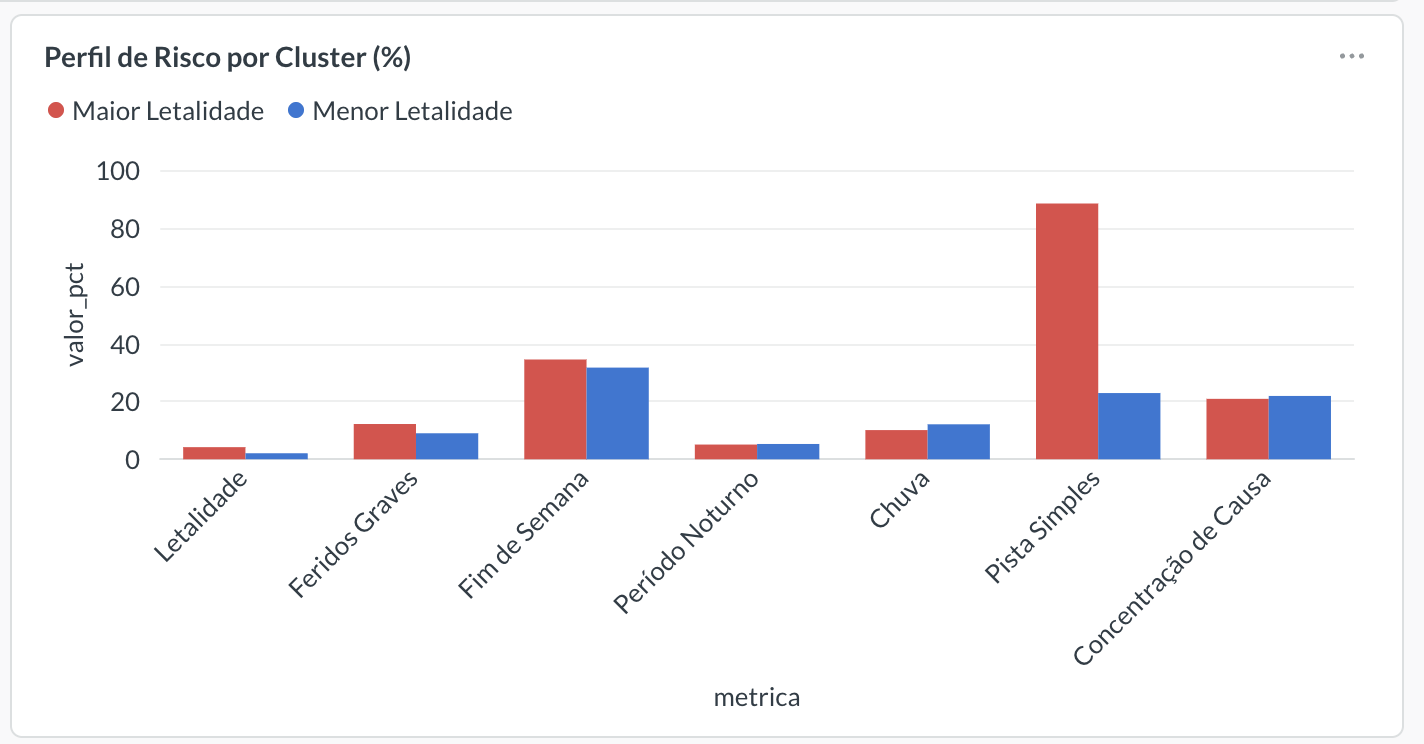
\includegraphics[width=0.6\textwidth]{./fig/perfil_risco_cluster}
  \caption{Card "Perfil de Risco por Cluster (\%)" no Metabase}
  \label{fig:metabase-perfil}
  \fontefig{Elaborado pelo autor, a partir do Metabase}
\end{figure}

\begin{figure}[H]
  \centering
  \begin{minipage}[t]{0.49\textwidth}
    \centering
    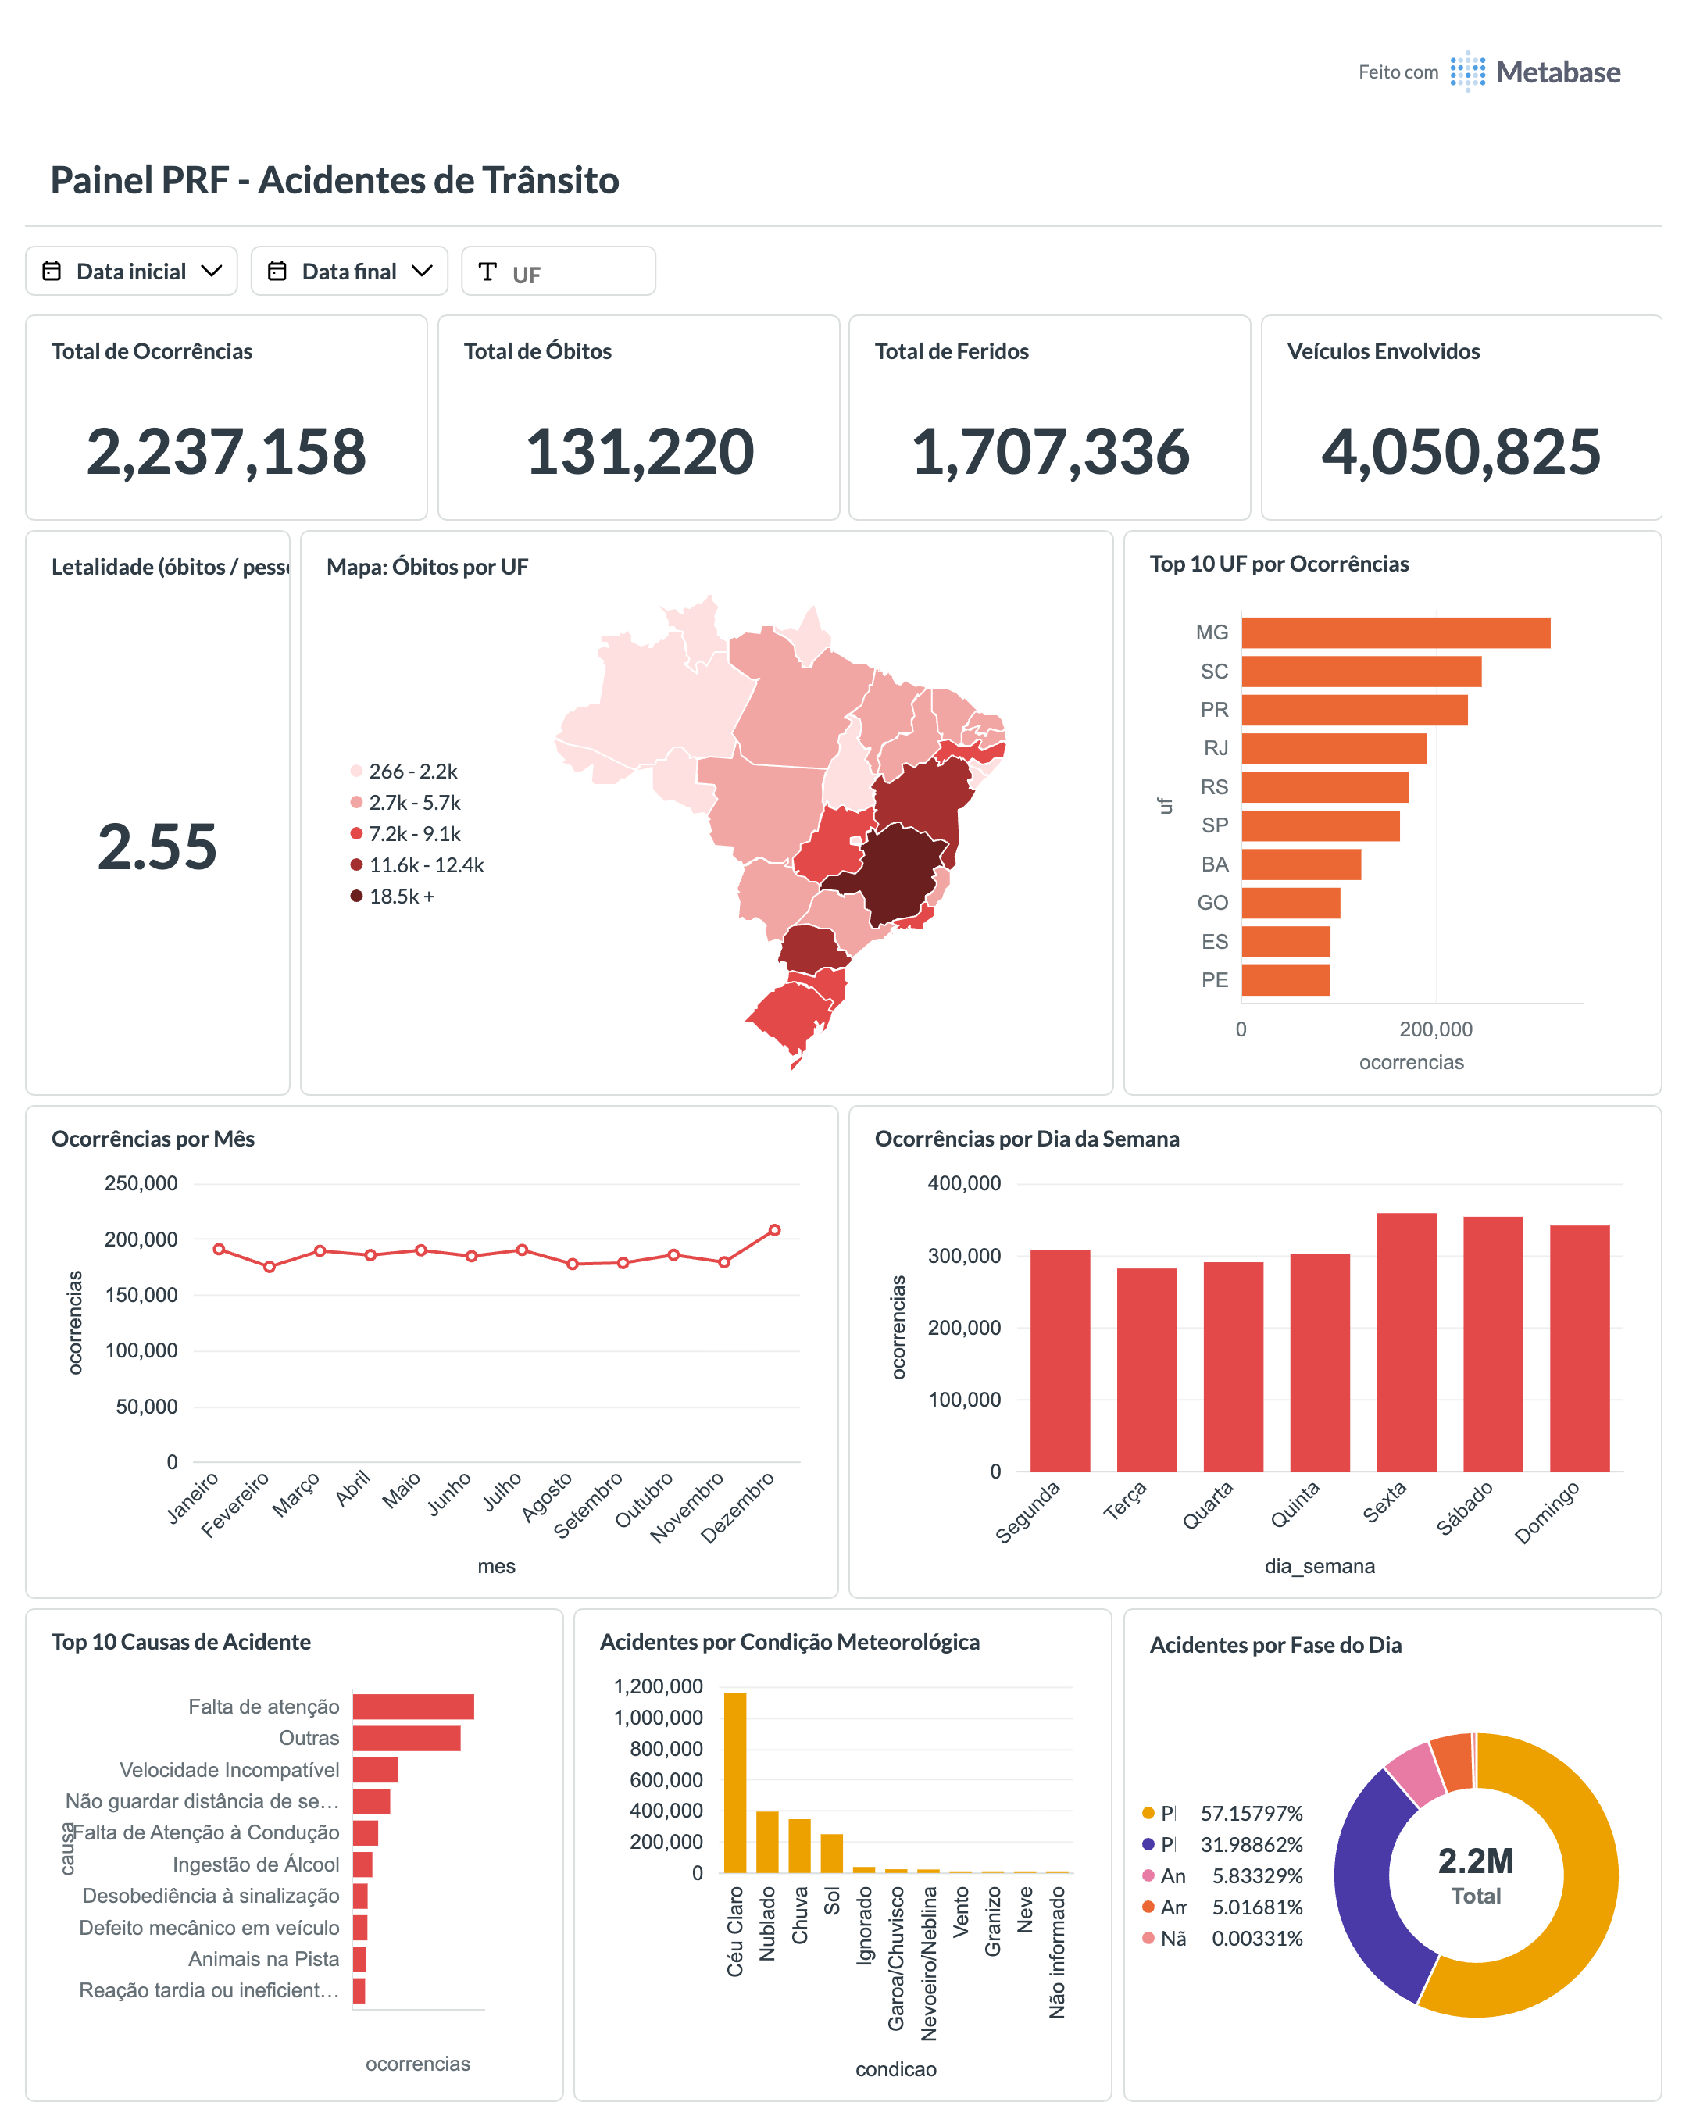
\includegraphics[page=1, width=\textwidth]{./fig/dashboard.pdf}
  \end{minipage}\hfill
  \begin{minipage}[t]{0.49\textwidth}
    \centering
    \includegraphics[page=2, width=\textwidth]{./fig/dashboard.pdf}
  \end{minipage}

  \vspace{0.3cm}
  \includegraphics[page=3, trim=7pt 636pt 7pt 7pt, clip, width=0.9\textwidth]{./fig/dashboard.pdf}
  \caption{Painel PRF - Acidentes de Trânsito no Metabase (exportação completa: três partes)}
  \label{fig:metabase-painel}
  \fontefig{Elaborado pelo autor, a partir do Metabase}
\end{figure}


